\documentclass[journal,12pt,twocolumn]{IEEEtran}

\usepackage{setspace}
\usepackage{gensymb}

\singlespacing


\usepackage[cmex10]{amsmath}

\usepackage{amsthm}

\usepackage{mathrsfs}
\usepackage{txfonts}
\usepackage{stfloats}
\usepackage{bm}
\usepackage{cite}
\usepackage{cases}
\usepackage{subfig}

\usepackage{longtable}
\usepackage{multirow}

\usepackage{enumitem}
\usepackage{mathtools}
\usepackage{steinmetz}
\usepackage{tikz}
\usepackage{circuitikz}
\usepackage{verbatim}
\usepackage{tfrupee}
\usepackage[breaklinks=true]{hyperref}
\usepackage{graphicx}
\usepackage{tkz-euclide}

\usetikzlibrary{calc,math}
\usepackage{listings}
    \usepackage{color}                                            %%
    \usepackage{array}                                            %%
    \usepackage{longtable}                                        %%
    \usepackage{calc}                                             %%
    \usepackage{multirow}                                         %%
    \usepackage{hhline}                                           %%
    \usepackage{ifthen}                                           %%
    \usepackage{lscape}     
\usepackage{multicol}
\usepackage{chngcntr}

\DeclareMathOperator*{\Res}{Res}

\renewcommand\thesection{\arabic{section}}
\renewcommand\thesubsection{\thesection.\arabic{subsection}}
\renewcommand\thesubsubsection{\thesubsection.\arabic{subsubsection}}

\renewcommand\thesectiondis{\arabic{section}}
\renewcommand\thesubsectiondis{\thesectiondis.\arabic{subsection}}
\renewcommand\thesubsubsectiondis{\thesubsectiondis.\arabic{subsubsection}}


\hyphenation{op-tical net-works semi-conduc-tor}
\def\inputGnumericTable{}                                 %%

\lstset{
%language=C,
frame=single, 
breaklines=true,
columns=fullflexible
}
\begin{document}


\newtheorem{theorem}{Theorem}[section]
\newtheorem{problem}{Problem}
\newtheorem{proposition}{Proposition}[section]
\newtheorem{lemma}{Lemma}[section]
\newtheorem{corollary}[theorem]{Corollary}
\newtheorem{example}{Example}[section]
\newtheorem{definition}[problem]{Definition}

\newcommand{\BEQA}{\begin{eqnarray}}
\newcommand{\EEQA}{\end{eqnarray}}
\newcommand{\define}{\stackrel{\triangle}{=}}
\bibliographystyle{IEEEtran}
\providecommand{\mbf}{\mathbf}
\providecommand{\pr}[1]{\ensuremath{\Pr\left(#1\right)}}
\providecommand{\qfunc}[1]{\ensuremath{Q\left(#1\right)}}
\providecommand{\sbrak}[1]{\ensuremath{{}\left[#1\right]}}
\providecommand{\lsbrak}[1]{\ensuremath{{}\left[#1\right.}}
\providecommand{\rsbrak}[1]{\ensuremath{{}\left.#1\right]}}
\providecommand{\brak}[1]{\ensuremath{\left(#1\right)}}
\providecommand{\lbrak}[1]{\ensuremath{\left(#1\right.}}
\providecommand{\rbrak}[1]{\ensuremath{\left.#1\right)}}
\providecommand{\cbrak}[1]{\ensuremath{\left\{#1\right\}}}
\providecommand{\lcbrak}[1]{\ensuremath{\left\{#1\right.}}
\providecommand{\rcbrak}[1]{\ensuremath{\left.#1\right\}}}
\theoremstyle{remark}
\newtheorem{rem}{Remark}
\newcommand{\sgn}{\mathop{\mathrm{sgn}}}
\providecommand{\abs}[1]{\left\vert#1\right\vert}
\providecommand{\res}[1]{\Res\displaylimits_{#1}} 
\providecommand{\norm}[1]{\left\lVert#1\right\rVert}
%\providecommand{\norm}[1]{\lVert#1\rVert}
\providecommand{\mtx}[1]{\mathbf{#1}}
\providecommand{\mean}[1]{E\left[ #1 \right]}
\providecommand{\fourier}{\overset{\mathcal{F}}{ \rightleftharpoons}}
%\providecommand{\hilbert}{\overset{\mathcal{H}}{ \rightleftharpoons}}
\providecommand{\system}{\overset{\mathcal{H}}{ \longleftrightarrow}}
	%\newcommand{\solution}[2]{\textbf{Solution:}{#1}}
\newcommand{\solution}{\noindent \textbf{Solution: }}
\newcommand{\cosec}{\,\text{cosec}\,}
\providecommand{\dec}[2]{\ensuremath{\overset{#1}{\underset{#2}{\gtrless}}}}
\newcommand{\myvec}[1]{\ensuremath{\begin{pmatrix}#1\end{pmatrix}}}
\newcommand{\mydet}[1]{\ensuremath{\begin{vmatrix}#1\end{vmatrix}}}
\numberwithin{equation}{subsection}
\makeatletter
\@addtoreset{figure}{problem}
\makeatother
\let\StandardTheFigure\thefigure
\let\vec\mathbf
\renewcommand{\thefigure}{\theproblem}
\def\putbox#1#2#3{\makebox[0in][l]{\makebox[#1][l]{}\raisebox{\baselineskip}[0in][0in]{\raisebox{#2}[0in][0in]{#3}}}}
     \def\rightbox#1{\makebox[0in][r]{#1}}
     \def\centbox#1{\makebox[0in]{#1}}
     \def\topbox#1{\raisebox{-\baselineskip}[0in][0in]{#1}}
     \def\midbox#1{\raisebox{-0.5\baselineskip}[0in][0in]{#1}}
\vspace{3cm}
\title{Assignment 8}
\author{R.OOHA}
\maketitle
\newpage
\bigskip
\renewcommand{\thefigure}{\theenumi}
\renewcommand{\thetable}{\theenumi}
%
\section{Question No.VECTORS-2.4}
\item Show that the points 
$\vec{A} = \myvec{2 \\ -1 \\ 1},\vec{B}=\myvec{1 \\ -3\\-5},\vec{C}=\myvec{3\\-4\\-4}$
are the vertices of a right angle triangle
%
\section{SOLUTION}
The direction vectors of $\vec{AC}$ and $\vec{BC}$ are 
\item 
\begin{align}
\vec{A-C}=\myvec{-1\\3\\5}\label{2.0.1}
\end{align}
\begin{align}
\vec{B-C}=\myvec{-2\\1\\-1}\label{2.0.2}
\end{align}
If $\vec{A}$,$\vec{B}$,$\vec{C}$ form a line,then,$\vec{AC}$ and $\vec{BC}$ should have the same direction vector.Hence,there exists a k such that 
\begin{align}
\vec{A-C}=k\myvec{\vec{B-A}}
\\
\implies \vec{A}=\frac{k\vec{B+C}}{k+1}
\end{align}
Since
\begin{align}
\vec{B-A} \neq k\myvec{\vec{B-C}}
\end{align}
the points are not colinear and form a traingle.An alternative method is to create the matrix.
\begin{align}
\vec{M}=\myvec{\vec{A-C}&\vec{B-C}}^\top
\end{align}
If $rank\myvec{\vec{M}}=1$,the points are colinear. The rank of a matrix is the number of nonzero rows left after doing row operations.In this problem,
\begin{align}
\vec{M}=\myvec{-1 & 3 &5 \\ -2 & 1 & -1}\xleftrightarrow{R_2 \rightarrow R_2-2R_1}
\myvec{-1 & 3 & 5\\ 0 & -5 & -11}
\\
\implies rank\myvec{\vec{M}}=2
\end{align}
as the number of non zero rows is 2 and the following figure represents the triangle formed by given points A,B and C
\\
PLOT OF GIVEN -
\begin{figure}[ht]
\centering
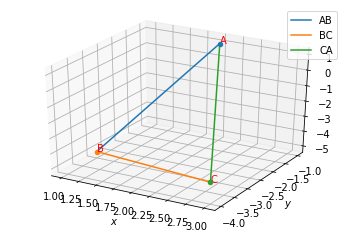
\includegraphics[width=\columnwidth]{Right angle triangle.png}
\caption{The right angle triangle}
\label{fig: The right angle triangle.}
\end{figure} 
From the figure,it appears that $\triangle\vec{ABC}$ is right angled,with $\vec{AB}$ as the hypotenuse.From Baudhayana's theorem,this would be true if
\begin{align}
\norm{\vec{A-C}}^2+\norm{\vec{B-C}}^2=\norm{\vec{A-B}}^2  
\end{align}
which can be expressed as
\begin{align}
\begin{split}
\norm{\vec{A}}^2+\norm{\vec{C}}^2-2\vec{A}^\top\vec{C}+\norm{\vec{B}}^2+\norm{\vec{C}}^2-2\vec{B}^\top\vec{C}\\
=\norm{\vec{A}}^2+\norm{\vec{B}}^2-2\vec{A}^\top\vec{B}
\end{split}
\end{align}
to obtain
\begin{align} \myvec{\vec{A-C}}^\top\myvec{\vec{B-C}}=0 \label{2.0.11}
\end{align}
after simplification.From $\eqref{2.0.1}$ and $\eqref{2.0.2}$,it is easy to verify that
\begin{align}
\myvec{\vec{A-C}}^\top\myvec{\vec{B-C}}=\myvec{-1&3&5}\myvec{-2\\1\\-1}\\=0
\end{align}
satisfying $\eqref{2.0.11}$.Thus,$\triangle \vec{ABC}$ is right angled at $\vec{C}$
\end{enumerate}
\end{document}